\documentclass[PhD]{PHlab-thesis}
\reversemarginpar        % 避免錯誤;不關心邊註方向時可保留
\setlength{\marginparwidth}{0pt}   % 邊註寬度設 0
\setlength{\marginparsep}{0pt}     % 邊註與正文的間距也設 0
\addbibresource{thesis.bib}

\newcommand*\Department中文{資訊工程學系}
\newcommand*\Department英文{Department of Computer Science and Information Engineering}

\newcommand*\ThesisTitle中文{WebGPU 於高效能生物資訊計算:瀏覽器端 Pair-HMM Forward 演算法之優化}
\newcommand*\ThesisTitle英文{ WebGPU for High-Performance Bioinformatics Computing: Browser-Based Optimization of the Pair-HMM Forward Algorithm}

\newcommand*\Student中文{王尊緯}
\newcommand*\Student英文{Tsun-Wei Wang}

\newcommand*\Advisor中文{賀保羅}
\newcommand*\Advisor英文{Paul Horton}

%% 果有共同指導老師可以用:
%% \newcommand*\CoAdvisorA中文{}
%% \newcommand*\CoAdvisorA英文{}
%% \newcommand*\CoAdvisorB中文{}
%% \newcommand*\CoAdvisorB英文{}


\newcommand*\YearMonth英文{July, 2025}
\newcommand*\YearMonth中文{114年7月}

\pagestyle{fancy}% Use fancyhdr

\usepackage{fancyhdr}
\pagestyle{fancy}
\setlength{\headheight}{13.6pt}
\renewcommand{\chaptermark}[1]{\markboth{Chapter \thechapter.\ #1}{}}
\fancyhead{}

\fancyhead[C]{\small\MakeUppercase{\leftmark}}


\begin{document}


% ---------- Keywords ----------
\newcommand*\Keywords英文{WebGPU, Pair-Hidden Markov Model, Bioinformatics Acceleration}
\newcommand*\Keywords中文{瀏覽器 GPU 計算、Pair-Hidden Markov Model (Pair-HMM)、生物資訊加速}

% ---------- Abstract (English) ----------
% ---------- Abstract (English) ----------
\newcommand*\Abstract英文{%
As GPU acceleration becomes increasingly prevalent in bioinformatics (Banerjee \emph{et al}., 2017; Liu \emph{et al}., 2021), conventional CUDA/OpenCL solutions still require driver installation and are locked to specific hardware, hindering online teaching and front-end clinical analysis. Ratified in 2024, \textbf{WebGPU} unifies Vulkan, Direct3D 12, and Metal behind a single JavaScript API (W3C, 2024), offering three decisive advantages: zero installation, cross-hardware portability, and on-device data residency. Using the compute-intensive Pair-Hidden Markov Model Forward (Pair-HMM Forward) algorithm (Durbin \emph{et al}., 1998) as a case study, we assess the performance and viability of this new framework.

Starting from Chou, Yu-Chen 's (2024) open-source C++/CUDA implementation (Chou, 2024), we first develop a WebGPU baseline version. We then tackle its primary bottlenecks—frequent CPU$\leftrightarrow$GPU round-trips and costly BindGroup reconstruction—by successively introducing: (i) single-\emph{CommandBuffer} batch submission and (ii) Dynamic Uniform Offsets. This leads to an optimized implementation referred to as \emph{WebGPU-Optimized}.

Across an NVIDIA RTX 2070 Super, Apple M1, and Intel UHD 620, and for sequence lengths from $10^{2}$ to $10^{5}$, the optimized version achieves notable speed-ups (exceeding $100\times$ in the best case) and attains over 80 \% of CUDA 's throughput. The relative log-likelihood error remains below $10^{-5}$ on all devices. Even without access to an NVIDIA GPU, our method still outperforms single-threaded C++ by one to two orders of magnitude.

These results demonstrate that pure JavaScript and WGSL can compute Pair-HMM Forward within seconds in a browser. We contribute two browser-specific optimization strategies and detailed cross-hardware measurements, laying the groundwork for Web-native genomic analysis tools and supporting the democratization and real-time execution of bioinformatics workloads.
}

% ---------- Abstract (Chinese) ----------
\newcommand*\Abstract中文{%
隨著 GPU 加速在生物資訊領域日漸普及(Banerjee 等,2017;Liu 等,2021),傳統 CUDA/OpenCL 解決方案必須安裝驅動且受限於特定硬體,對線上教學與臨床前端分析造成不便。2024 年正式標準化的 WebGPU 以單一 JavaScript API 對接 Vulkan/D3D12/Metal(W3C,2024),兼具「免安裝、跨硬體、資料留在本機」三大優勢。本研究以高強度 Pair-Hidden Markov Model Forward(Pair-HMM Forward)演算法(Durbin 等,1998)為例,評估 WebGPU 的效能與可行性。

我們以周育晨(2024)公開之 C++/CUDA 程式為基準(Chou,2024),首先撰寫 WebGPU Baseline;接著針對 CPU↔GPU 往返與 BindGroup 重建等瓶頸,依序導入「單一 CommandBuffer 批次提交」與「Dynamic Uniform Offset」,形成 \emph{WebGPU-Optimized}。於 NVIDIA RTX 2070 Super、Apple M1 與 Intel UHD 620 針對序列長度 $10^{2}$--$10^{5}$ 之測試顯示,Optimized 相較 Baseline 能顯著加速(最高逾百倍),執行速度可達 CUDA 的八成以上;三款裝置的 log-likelihood 相對誤差皆低於 $10^{-5}$,且在無 NVIDIA GPU 時仍對單執行緒 C++ 提供數十至數百倍的加速。

本研究證實僅憑 JavaScript 與 WGSL,即能於瀏覽器中在秒級完成 Pair-HMM Forward 計算,並提出兩項瀏覽器端專屬優化策略及跨硬體實測結果。此成果為 Web-native 基因體分析工具的普及奠定基礎,推動生物資訊運算的民主化與即時化。
}



\newcommand*\Acknowledgements{%
在此特別感謝賀保羅教授以及在實驗室給予我協助與指導的同學:阮祈翰、楊祐昇、黃書堯、鄭驊軒、鄭煜醴等,在各階段實驗設計與資料收集上提供許多寶貴意見。

同時感謝林宜靜、賴威達、王晴文、許庸袁及陳竑曄,你們在討論分析與程式測試時的協作與支持,讓本研究得以順利完成。

最後,感謝所有關心及協助本研究的師長與同窗,謹此致上由衷謝意。 }



\newcommand*\SelectFontsize[2]{\fontsize{#1}{#1}\selectfont\mdseries#2\par}
\newcommand*\SelectFontsizeBF[2]{\fontsize{#1}{#1}\selectfont\bfseries#2\par}
\newcommand*\SignatureRule[1][6]{\rule{#1cm}{0.3mm}}
\newcommand*\AddToContents[1]{\newpage\phantomsection\addcontentsline{toc}{chapter}{#1}}

\doublespace
\pagenumbering{gobble}
\renewcommand{\thefootnote}{\fnsymbol{footnote}}


\begin{center}
\vspace{2cm}
\SelectFontsizeBF{24}{%
\University中文\Department中文\\
\學位 論文}

\vfill
\SelectFontsizeBF{24}{\ThesisTitle中文}
\ifdefined\ThesisNote中文
\SelectFontsize{22}{\textit{\ThesisNote中文}}
\fi

\vspace{5mm}
\SelectFontsizeBF{22}{\ThesisTitle英文}
\ifdefined\ThesisNote英文
\SelectFontsize{20}{\textit{\ThesisNote英文}}
\fi

\vfill

\begin{minipage}{\linewidth}
{\setlength\tabcolsep{0pt}
%
\begin{tabular}{ Wr{5em} Wl{6em} Wr{5em} wl{7em} }
研究生:   & ~~\Student中文  &      Student: & ~~\Student英文\\
指導老師: & ~~\Advisor中文  &      Advisor: & ~~\Advisor英文\\
\ifdefined\CoAdvisorA中文
共同指導: & ~~\CoAdvisorA中文 &   Co-Advisor: & ~~\CoAdvisorA英文\\
\fi
\ifdefined\CoAdvisorB中文
         & ~~\CoAdvisorB中文 &   Co-Advisor: & ~~\CoAdvisorB英文\\
\fi
\end{tabular}
}
\end{minipage}

\vfill
\SelectFontsize{18}{%
National Cheng Kung University,\\
Tainan, Taiwan, R.O.C.\\
Thesis for \ifdef\PhD{Master of Science}{Doctor of Philosophy} Degree\\
\YearMonth英文}

\vfill
\SelectFontsize{20}{中華民國\YearMonth中文}
\end{center}



\ifdefined\optCommittee
\newpage
\begin{center}
\vspace{1cm}
\SelectFontsizeBF{24}{%
\University中文\Department中文\\
\學位 論文}
\vfill
\SelectFontsizeBF{20}{\ThesisTitle中文}
\end{center}

\vfill
\SelectFontsize{20}{%
\noindent 研究生:\Student中文\\
本論文業經審查及口試合格特此證明}


\begin{center}
\SelectFontsize{18pt}{論文考試委員}
\vfill
\SignatureRule \hspace*{1cm} \SignatureRule
\vfill

\SignatureRule \hspace*{1cm} \SignatureRule
\vfill

指導教授:\SignatureRule[8]
\vfill
  所長:\SignatureRule[8]

\vfill
\SelectFontsize{18}{中華民國 \hspace{2em} 年 \hspace{2em} 月 \hspace{2em} 日}
\end{center}


\newpage
\begin{center}
\vspace{1cm}
\SelectFontsize{18}{\University英文, \Department英文}
\SelectFontsize{19}{\ifdef\PhD{Ph.D.}{Master's} Degree Thesis}

\vfill
\SelectFontsizeBF{20}{\ThesisTitle英文}
\end{center}

\vfill
\SelectFontsize{18}{Student: \Student英文}

\SelectFontsize{18}{%
A thesis submitted to the graduate division in partial fulfillment of the requirement for the degree of
\ifdef\PhD{Master of Science}{Doctor of \mbox{Philosophy}}.
}

\vfill
\begin{center}
\SelectFontsize{18}{Approved by}

\vfill
\SignatureRule \hspace*{1cm} \SignatureRule

\vfill
\SignatureRule \hspace*{1cm} \SignatureRule

\vfill
Advisor: \SignatureRule[8]

\vfill
Chairman: \SignatureRule[8]

\vfill
\SelectFontsize{18}{\YearMonth英文}
\vspace*{20pt}
\end{center}
\fi% optCommittee


\AddToContents{中文摘要}
\setcounter{page}{1}
\pagenumbering{roman}


\begin{center}
\SelectFontsizeBF{24}{\ThesisTitle中文}

\vspace{4mm}
\SelectFontsize{18}{\Student中文\footnote[1]{學生} ~ \Advisor中文\footnote[2]{指導教授}}

\vspace{5mm}
\SelectFontsize{20}{國立成功大學\Department中文}

\vspace{12mm}
\makebox[2.7cm][c]{\SelectFontsizeBF{22}{摘要}}
\end{center}

\vspace{4mm}
\SelectFontsize{16}{\Abstract中文}

\vspace{4mm}
\begin{flushleft}
\SelectFontsize{16}{\textbf{關鍵詞:} \Keywords中文}
\end{flushleft}



\AddToContents{Abstract}
\begin{center}
\SelectFontsizeBF{22}{\ThesisTitle英文}

\vspace{4mm}
\SelectFontsize{18}{\Student英文\footnote[1]{Student} ~ \Advisor英文\footnote[2]{Advisor}}

\vspace{4mm}
\SelectFontsize{16}{\Department英文, National Cheng Kung University}

\vspace{12mm}
\SelectFontsizeBF{20}{Abstract}
\end{center}

\vspace{4mm}
\SelectFontsize{14}{\Abstract英文}

\vspace{4mm}
\begin{flushleft}
\SelectFontsize{16}{\textbf{Keywords:} \Keywords英文}
\end{flushleft}



\AddToContents{誌謝}
\begin{center}\SelectFontsizeBF{24}{誌謝}\end{center}

\vspace{4mm}
\Acknowledgements



\renewcommand{\contentsname}{CONTENTS}
\AddToContents{Contents}
\tableofcontents


\AddToContents{List of Tables}
\listoftables


\AddToContents{List of Figures}
\listoffigures
% 封面頁, 口委中英文簽名單, 誌謝, 中英文摘要, 論文目錄, 圖表目錄


%────────────────────  List of Symbols  ────────────────────
\renewcommand\nomgroup[1]{%
  \item[\bfseries
  \ifstrequal{#1}{A}{General}{%
  \ifstrequal{#1}{Z}{Gene/Protein Names}%
  }]}

% === A. General ===
\nomenclature[A]{HPC}{High-Performance Computing}
\nomenclature[A]{API}{Application Programming Interface}
\nomenclature[A]{BWA}{Burrows–Wheeler Aligner}
\nomenclature[A]{GATK}{Genome Analysis Toolkit}

% === B. Algorithm / Computational Model ===
\nomenclature[B]{HMM}{Hidden Markov Model}
\nomenclature[B]{SIMD}{Single Instruction Multiple Data}
\nomenclature[B]{FMA}{Fused Multiply-Add instruction}
\nomenclature[B]{SM}{Streaming Multiprocessor (CUDA core block)}
\nomenclature[B]{LUT}{Lookup Table}

% === C. GPU / WebGPU & Related Technologies ===
\nomenclature[C]{CUDA}{Compute Unified Device Architecture}
\nomenclature[C]{OpenCL}{Open Computing Language}
\nomenclature[C]{WASM}{WebAssembly}
\nomenclature[C]{WASM-SIMD}{SIMD extension of WebAssembly}
\nomenclature[C]{WGPU}{Cross-platform WebGPU API implementation}
\nomenclature[C]{ALU}{Arithmetic Logic Unit}
\nomenclature[C]{UMA}{Unified Memory Architecture}
\nomenclature[C]{DRAM}{Dynamic Random-Access Memory}
\nomenclature[C]{TFLOPS}{Tera Floating-Point Operations per Second}
\nomenclature[C]{SDK}{Software Development Kit}


\printnomenclature[5cm]

\newpage
\setcounter{page}{1}
\pagenumbering{arabic}

\chapter{Introduction}

\section{Background}
High-throughput sequencing (Next-Generation Sequencing, NGS) has driven the exponential growth in both scale and complexity of genomic data (Mardis, 2017), creating unprecedented computational demands in bioinformatics. The \textbf{Pair Hidden Markov Model (Pair-HMM) Forward algorithm}—which supports sequence alignment, genotype calling, and variant detection—remains a core computation in many genomic pipelines (Durbin et al., 1998).

Current analysis workflows, such as GATK \cite{McKenna2010}, Samtools \cite{Li2009}, and BWA-MEM2 \cite{Vasimuddin2019}, are predominantly implemented in C++ or Python and rely on GPU acceleration via NVIDIA CUDA or OpenCL \cite{Liu2021,Banerjee2017}. However, this approach ties users to specific GPU vendors and requires installing proprietary drivers, SDKs, and dependencies. In teaching environments or resource-constrained laboratories, the lack of high-end GPUs or limited cloud quotas often forces a fallback to CPU execution, greatly inflating both cost and turnaround time. Even though cloud services simplify setup, they introduce account management overhead, network latency, and potential concerns about exposing sensitive data.

\section{Motivation and Objectives}
Since WebGPU’s official release in Chrome’s stable channel in May 2024 \cite{GoogleChromeDevs2024}, with experimental support in Firefox Nightly and Edge Dev, it has promised driver-free, cross-vendor GPU computing through a unified JavaScript API mapping Vulkan, Direct3D 12, and Metal (W3C, 2024). This development opens new opportunities for lowering the barrier to GPU-accelerated bioinformatics tools—especially in educational, clinical, and low-resource settings.  
Nonetheless, WebGPU was designed primarily for graphics and ML inference, and running a compute-intensive dynamic programming algorithm like Pair-HMM Forward presents several key challenges:
\begin{itemize}
    \item \emph{API scheduling overhead} – Processing wavefronts sequentially incurs CPU–GPU round trips when creating new \texttt{CommandBuffer} and \texttt{BindGroup} for each dispatch.
    \item \emph{Lack of global synchronization} – WebGPU provides only workgroup-level barriers and lacks CUDA-style kernel-return global sync \cite{W3C2024}.
    \item \emph{Absence of dedicated special-function units (SFUs)} – Pair-HMM relies heavily on \texttt{log}/\texttt{exp} calls. While CUDA’s SFUs can compute \texttt{log\_2} in four cycles (NVIDIA, 2023), WebGPU must approximate these using ALU, lookup tables, and FMA, incurring a 2–4× latency penalty.
    \item \emph{High memory-access demand} – The DP matrix resides in a read-write storage buffer; WebGPU’s default path bypasses L1 cache, so frequent global reads and writes generate substantial DRAM traffic \cite{Liu2021}.
\end{itemize}
To assess WebGPU’s practical viability for bioinformatics, we pose the central question: \emph{Can WebGPU inside a browser execute the Pair-HMM Forward algorithm with performance comparable to CUDA?}

\section{Methods and Key Results}
Building on the open-source C++/CUDA reference implementation by Chou \cite{chou2024}, we introduce two browser-specific optimizations to mitigate the above bottlenecks:
\begin{enumerate}
    \item \emph{Batch submission with a single \texttt{CommandBuffer}} – Aggregating multiple wavefronts into one \texttt{queue.submit()} call to eliminate repeated API round-trip latency.
    \item \emph{Dynamic Uniform Offsets} – Storing static parameters in a single uniform buffer and accessing them via dynamic offsets to avoid multiple UBO allocations and bindings.
\end{enumerate}
On an NVIDIA RTX 2070 Super with sequence lengths from 100 to 100 000, our “WebGPU-Optimized” implementation achieves 6.8–142× speedups over the CPU baseline and attains 11–84\% of CUDA’s throughput. On Apple M1 and Intel UHD 620 GPUs for sequences ≥1 000, it delivers 4–463× speedups while maintaining log-likelihood errors below $10^{-5}$.

\section{Conclusions and Contributions}
This study demonstrates that JavaScript combined with WGSL can solve medium-to-large Pair-HMM Forward instances in seconds within a browser sandbox. Our two complementary optimizations effectively mitigate API, synchronization, and memory bottlenecks, and cross-vendor evaluation on NVIDIA, Apple, and Intel GPUs confirms hardware agnosticism. These results pave the way for “open-the-browser-and-compute” genomic analysis and provide an empirical foundation for future work on double-precision support and WASM-SIMD + WebGPU hybrid acceleration.



\chapter{Related Work}

\section{High-Performance Computing Requirements in Bioinformatics}

\subsection{Next-Generation Sequencing and Its Computational Challenges}
Next-Generation Sequencing (NGS) has driven an exponential increase in genomic data volume \cite{Mardis2017}. For instance, an Illumina NovaSeq X Plus with a 25 B flow cell in dual-lane mode can generate approximately \(5.2\times10^{10}\) paired-end reads (2 × 150 bp) over a 48 h run—about \(3.25\times10^{11}\) bases per hour \cite{Illumina2024}. Such data throughput far exceeds the capabilities of traditional CPU-only architectures for downstream analyses.

Alignment tools like BWA \cite{LiDurbin2010} and Bowtie \cite{Langmead2009} routinely process millions to billions of short reads. Although their worst-case time complexity is \(O(NM)\), FM-index–based seeding and extension typically yield near-linear average cost \(O(L)\) in read length \(L\) \cite{FerraginaManzini2000}. These computational demands have driven the adoption of high-performance computing (HPC) solutions—particularly GPU acceleration—to meet real-time requirements in modern bioinformatics pipelines \cite{Liu2021}.

\subsection{The Central Role of the Pair-HMM Forward Algorithm}
The Pair-Hidden Markov Model (Pair-HMM) Forward algorithm underlies key operations in sequence alignment and genotype inference, powering tools such as GATK \cite{McKenna2010} and Samtools \cite{Li2009}. As Durbin et al. \cite{Durbin1998} describe, its time complexity is \(O(NM)\) with memory footprint reducible to \(O(\max\{N,M\})\). For long reads (\(N\approx10^4\)), Pair-HMM Forward becomes a primary computational bottleneck. Recent work by Schmidt et al. \cite{Schmidt2024} demonstrates that GPU parallelisation can reduce processing time for 32\(\times\)12 kb fragments on an NVIDIA RTX 4090 from hours to under three minutes, highlighting both the potential and the sensitivity of the algorithm to memory-access patterns and numerical precision.

\section{Conventional GPU Acceleration Frameworks}

\subsection{CUDA in Bioinformatics}
NVIDIA CUDA has emerged as the de facto standard for GPU computing in bioinformatics. Liu et al. \cite{Liu2013} achieved 30–90× speedups for the Smith–Waterman algorithm with CUDASW++ 3.0 compared to single-threaded CPUs. Schmidt et al. \cite{Schmidt2024} further applied CUDA optimisations to the Pair-HMM Forward algorithm, attaining high throughput in large-scale genotyping workflows. Nonetheless, CUDA remains tied to NVIDIA hardware and requires proprietary driver and toolkit installations. Kernel tuning for specific microarchitectures (e.g., Ampere, Hopper) further limits portability across GPU generations.

\subsection{OpenCL’s Cross-Platform Ambition}
OpenCL was designed for hardware-agnostic GPU acceleration, supporting NVIDIA, AMD, and Intel devices \cite{Stone2010}. Klöckner et al. \cite{Klockner2012} demonstrated its utility in scientific computing, yet its adoption in bioinformatics lags behind CUDA due to inconsistent memory-management and thread-synchronisation behaviors across vendors \cite{Klockner2012}. The relative immaturity of the OpenCL ecosystem and the lack of a comprehensive bioinformatics library base further constrain its widespread use.

\section{Barriers and Limitations of Traditional Frameworks}
While CUDA and OpenCL deliver high performance, both impose intricate setup steps—driver installation, SDK configuration, and dependency management—that impede deployment in teaching environments and clinical front-ends. Cloud-based GPU services (e.g., AWS, Google Cloud) alleviate local setup burdens but introduce data-transfer latency and privacy concerns \cite{Krampis2012}. Moreover, neither framework offers seamless cross-platform compatibility on resource-constrained devices such as laptops or embedded systems, limiting their practicality for democratized bioinformatics computing.




\section{The Emergence and Technical Characteristics of WebGPU}

\subsection{Technical Background}
On 19 December 2024, WebGPU entered the W3C Candidate Recommendation Snapshot stage; it has not yet reached full Recommendation status and therefore still awaits complete implementations and interoperability tests (W3C, 2024). Figure~\ref{fig:webgpu-mapping} illustrates WebGPU's architecture: a single JavaScript / TypeScript API translates application calls to Vulkan, Direct3D 12, or Metal back ends, which are then dispatched to the underlying GPU. This design offers three major advantages—driver-free installation, cross-platform compatibility, and browser-sandbox safety (Google Chrome Developers, 2024).

WebGPU's compute pipeline is written in WGSL (WebGPU Shading Language), which supports high-performance matrix operations and explicit memory control (W3C, 2024), making it suitable for compute-intensive workloads.

\begin{figure}[htbp]
    \centering
    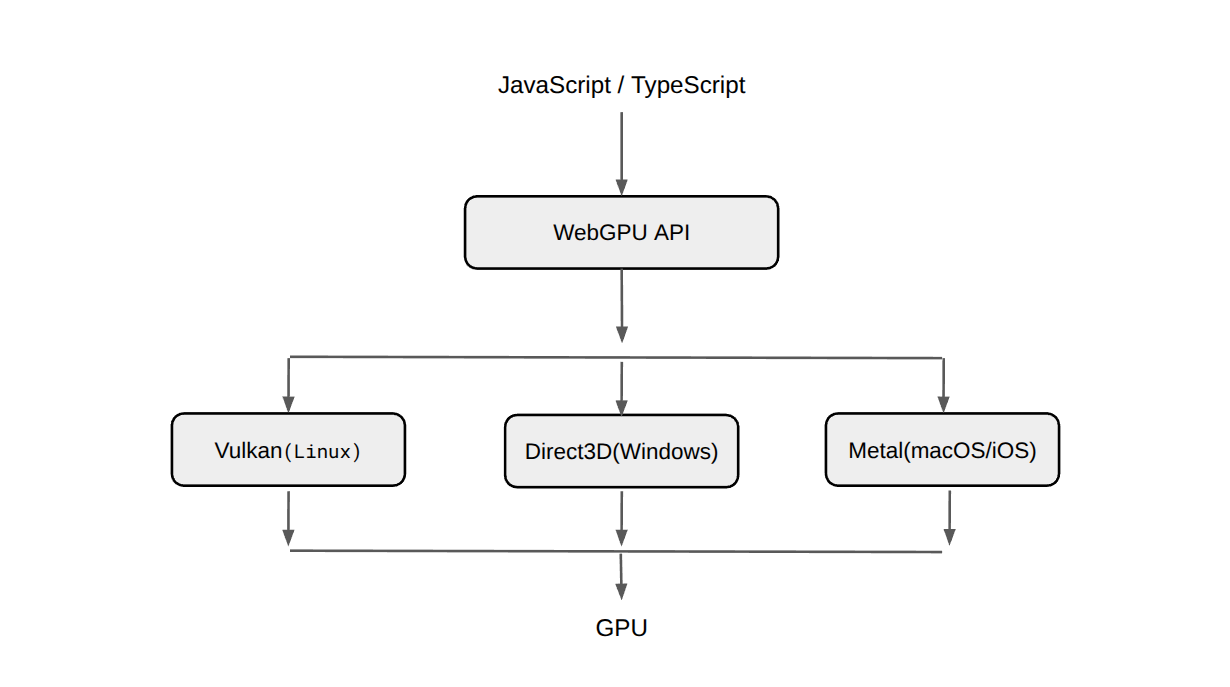
\includegraphics[width=0.9\linewidth]{WebGPU 架構對應示意.png}
    \caption{Mapping between the WebGPU API and native back ends}
    \label{fig:webgpu-mapping}
\end{figure}

JavaScript/TypeScript invokes WebGPU through a unified interface. The browser selects Vulkan (Linux), Direct3D 12 (Windows), or Metal (macOS/iOS) as the actual back end and submits commands to the GPU.

\subsection{High-Performance Computing Potential of WebGPU}
WebGPU has already shown promise in graphics and machine-learning domains. MDN Web Docs (2025) reports game-rendering performance on WebGPU that rivals native Vulkan, while TensorFlow.js accelerates in-browser neural-network training via its WebGPU back end (TensorFlow.js Team, 2024). According to the Google Chrome Team (2024), Transformers.js running BERT-base on an NVIDIA RTX 4060 Laptop is 32.51$\times$ faster in WebGPU mode than in WebAssembly, underscoring WebGPU's performance potential.

These cases demonstrate that WebGPU's execution model can exploit GPU parallelism effectively. However, its adoption in bioinformatics remains nascent because the field demands stricter numerical precision and memory-access efficiency. WebGPU trades some low-level control for broad hardware portability, which distinguishes its compute shaders from those of traditional GPU frameworks.

\subsection{Challenges and Limitations of WebGPU}
Despite its cross-platform appeal, WebGPU still faces hurdles in high-intensity computing. First, browser-side API scheduling overhead is relatively high, particularly during frequent CPU–GPU data exchanges (Google Chrome Team, 2024). Second, WebGPU exposes only \texttt{workgroupBarrier} and lacks any cross-workgroup global-synchronisation primitive, hampering algorithms that require complex thread coordination (W3C, 2024).

Moreover, the browser sandbox constrains memory allocation and special-function-unit (SFU) usage. WGSL lacks built-in transcendental functions (e.g., \texttt{log}, \texttt{exp}) and must rely on software emulation; although the GPU may execute these via SFUs, additional overhead remains. Double-precision (\texttt{f64}) support is also less mature than in CUDA (Jones, 2023). The wavefront dependencies of Pair-HMM Forward demand frequent memory access and thread synchronisation, making high-performance parallelisation challenging under WebGPU's current limitations.

\section{Initial Explorations of WebGPU in Bioinformatics}
Direct WebGPU applications in bioinformatics are still scarce, but related technologies such as WebGL and WebAssembly (WASM) provide useful precedents. Ghosh \emph{et al}. (2018) used WebGL to build Web3DMol, showing that in-browser molecular visualisation is feasible and that JavaScript can serve bioinformatics needs. WASM-SIMD further boosts browser-side performance; Jones (2023) argues that combining WASM-SIMD with WebGPU could accelerate sequence processing.

Other compute-intensive domains also offer insights. For instance, the WebGPU back end of TensorFlow.js speeds up browser-based neural-network training through efficient matrix operations (TensorFlow.js Team, 2024); its memory-management and parallelisation strategies inspire our port of Pair-HMM Forward, particularly for handling frequent memory access and compute-heavy kernels. Nonetheless, existing studies focus mostly on visualisation or lightweight workloads; implementations of high-intensity algorithms such as Pair-HMM Forward remain unexplored. While Schmidt \emph{et al}. (2024) provide a CUDA baseline, they do not investigate browser-specific optimisations.

\section{Research Gap and Positioning of This Work}
The literature reveals three key shortcomings:
\begin{enumerate}
    \item Lack of systematic verification of WebGPU's performance and feasibility for compute-heavy bioinformatics tasks such as Pair-HMM Forward.
    \item Absence of browser-specific optimisation strategies addressing GPU-compute bottlenecks—CPU–GPU round-trips and BindGroup reconstruction, . For example, each \texttt{setBindGroup()} call traverses multiple layers (V8 $\rightarrow$ Blink $\rightarrow$ Dawn $\rightarrow$ Driver), incurring $\sim$5–15 $\mu$s of latency (Google Chrome Developers, 2024), which is significant for wavefront algorithms.
    \item Insufficient cross-hardware evaluations (NVIDIA, Apple, Intel) to gauge WebGPU's generality. Mainstream tools like GATK reference sequence Caller require CUDA and thus NVIDIA drivers, limiting deployment in classrooms or resource-constrained environments; cloud solutions raise latency and privacy concerns (Krampis \emph{et al}., 2012).
\end{enumerate}
By porting Chou, Yu-Chen's (2024) CUDA implementation to WebGPU, this study proposes two browser-side optimisations—\emph{single-CommandBuffer batch submission} and \emph{Dynamic Uniform Offsets} —and validates their performance and accuracy across multiple hardware platforms. The results close the research gap in WebGPU bioinformatics applications and lay the foundation for driver-free, cross-hardware, on-device genomic analysis tools.




\chapter{Methods}

\section{Synthetic Dataset Generation}\label{sec:dataset}
To evaluate the performance of the proposed GPU-accelerated Pair-HMM, we
dynamically generate four synthetic test datasets of 100, 1 000, 10 000,
and 100 000 bp immediately before each run.
For every length, the host CPU first constructs a
$\textit{len}\!\times\!4$ read-probability matrix whose nucleotide
probabilities (A, C, G, T) are all 0.25.
It then creates a reference sequence sequence of identical length consisting
entirely of the nucleotide “A”.
Both the read profile and the reference sequence are copied to the GPU, where the
forward algorithm is executed.
This design eliminates input-data randomness, enabling a focused
comparison of how different parallelisation strategies scale in
computational and memory efficiency as sequence length increases.

\paragraph{Provenance of the generator}%
The entire dataset-generation procedure—including the random
read-probability generator, transition matrix, and emission constants—was
ported \emph{verbatim} from the open-source C++/CUDA reference
implementation released by Yu-Chen~Chou\cite{chou2024}.
None of the dataset-generation code was written as part of this study; we
adopted the original implementation without modification.
Reusing the same logic ensures that both our WebGPU kernels and the CUDA
baseline process identical input data, enabling a fair and consistent
comparison.


\section{Mathematical Model}
This study adopts a Pair-HMM combined with a sequence profile, following
the formulation in~[2].

Hidden states are Match (M), Insert (I), and Delete (D) over the alphabet
$\{A,C,G,T,-\}$.

The read sequence is represented by a probability matrix
\[
P = [p_{i,a}], \quad 1 \le i \le m,\;
a \in \{A,C,G,T\},\;
\sum_a p_{i,a} = 1,
\]
giving the probability that position~$i$ of the read is character~$a$
[3].

The reference sequence is a fixed string $h_1,\dots,h_n$.

The transition probabilities
\[
t_{XY}, \quad X,Y \in \{M,I,D\},
\]
and the base-emission matrix $\varepsilon_X(x,y)$ use the same settings
as the reference implementation~[1].

For the \emph{Match} and \emph{Insert} states, the emission probability at
alignment cell~$(i,j)$ is obtained by taking a probability-weighted average
between the read-base distribution at position~$i$ and the corresponding
base-emission coefficients.  
The \emph{Delete} state always emits a gap, so its emission probability is~1.


\section{Pair-HMM Forward Algorithm}
The forward recursion advances along anti-diagonals (wavefronts) of the
dynamic-programming matrix, as illustrated in
Figure~\ref{fig:pairhmm-wavefront}.
Each wavefront can proceed only after the previous one completes;
without device-side global synchronisation, this dependency becomes a
performance bottleneck on the GPU [3].

\begin{enumerate}
  \item \textit{Initialisation}
  \[
    M_{0,j} = I_{0,j} = 0,\quad D_{0,j} = \frac{1}{n}\quad(j>0).
  \]
  \item \textit{Recursion} [2]
  \[
    M_{i,j} = e_{i,j}^{M}\bigl(t_{MM}M_{i-1,j-1} + t_{IM}I_{i-1,j-1}
               + t_{DM}D_{i-1,j-1}\bigr),
  \]
  \[
    I_{i,j} = e_{i,j}^{I}\bigl(t_{MI}M_{i-1,j} + t_{II}I_{i-1,j}\bigr),
  \]
  \[
    D_{i,j} = t_{MD}M_{i,j-1} + t_{DD}D_{i,j-1}.
  \]
  \item \textit{Termination}
  \[
    P = \sum_{j=1}^{n}\bigl(M_{m,j} + I_{m,j}\bigr).
  \]
  \item \textit{Time complexity} is $\mathcal{O}(nm)$.
\end{enumerate}

\begin{figure}[htbp]
  \centering
  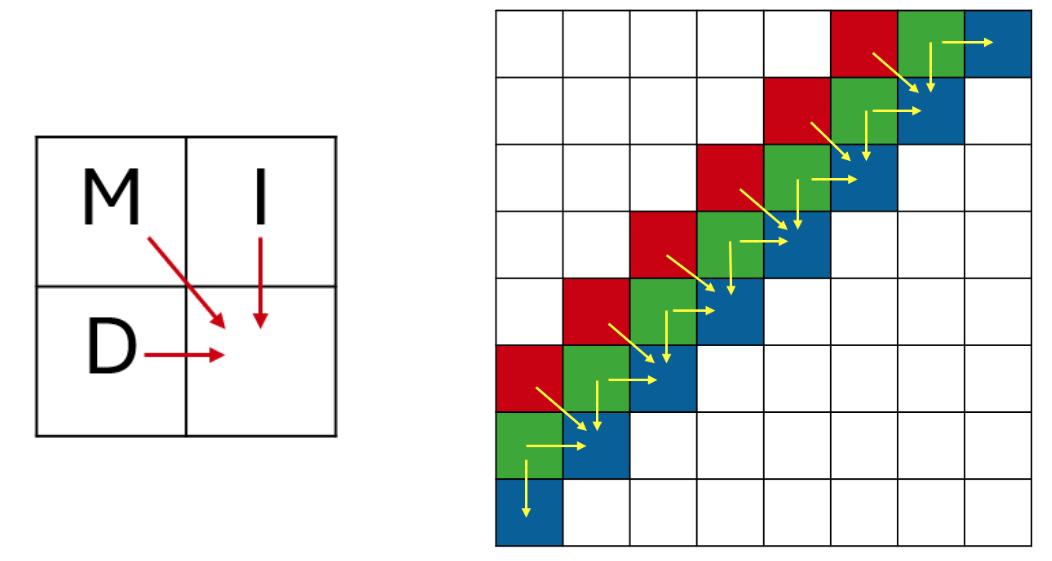
\includegraphics[width=0.9\linewidth]
    {Pair-HMM Forward 的計算沿反對角線 .png}
  \caption{Wavefront computation in the Pair-HMM Forward algorithm}
  \label{fig:pairhmm-wavefront}
\end{figure}


\section{System Design and Implementation}

\subsection{C++/CUDA Version}
Building on prior work showing CUDA can efficiently implement Pair-HMM via anti-diagonal parallelisation (Banerjee \emph{et al}., 2017; Schmidt \emph{et al}., 2024), we adopted and refactored the open-source C++/CUDA code by Chou, Yu-Chen (2024). All double-precision (\texttt{double}) variables were converted to single precision (\texttt{float}) so that the CUDA results represent an upper-bound “performance ceiling” directly comparable with our WebGPU implementation. Because WebGPU currently guarantees only \texttt{f32} arithmetic (W3C, 2024), retaining \texttt{f64} on CUDA would have obscured cross-platform comparisons with precision differences. After conversion, the maximum relative error at sequence length $N = 10^{5}$ was merely $2.18 \times 10^{-1}\%$, satisfying the accuracy threshold for subsequent WebGPU validation.

We preserve the “one kernel per anti-diagonal” structure: each of the $2N$ wavefronts launches a kernel, and a \texttt{cudaDeviceSynchronize()} between adjacent wavefronts acts as a GPU-wide barrier to ensure all thread-block dependencies are fully resolved (NVIDIA, 2023). This maps the DP-recurrence dependencies on the left, above, and upper-left cells to device execution in the most straightforward manner.

Global synchronisation alone, however, cannot hide memory latency. Inside each block we therefore keep a fine-grained \texttt{\_\_syncthreads()} barrier so that every 32 threads share cached values from the previous row before advancing. For the three DP arrays $M$, $I$, and $D$, we employ a host-side “four-row pointer rotation”: four $(n\!+\!1)$-length buffers are allocated once, and the host loop rotates pointers to realise the \texttt{prev $\rightarrow$ curr $\rightarrow$ new} shift (Liu, Wirawan, \& Schmidt, 2013). Because CUDA pointers can be treated as ordinary C pointers, this scheme avoids reallocations and \texttt{memcpy} overhead, maximising effective PCIe/NVLink bandwidth.

This structure also paves the way for the WebGPU port: once inside the browser we lose mutable pointers and must replace them with either BindGroup reconstruction or Dynamic Uniform Offsets (Google Chrome Developers, 2024).




\subsection{WebGPU Baseline}

\subsubsection{From CUDA “multiple kernels” to WebGPU “multiple dispatches”}
Pair-HMM Forward advances along anti-diagonals (wavefronts); each wavefront must finish before the next can begin (Durbin \emph{et al}., 1998).

The most straightforward CUDA strategy is a host-side \texttt{for} loop that launches successive kernels and inserts a \texttt{cudaDeviceSynchronize()} between them—an approach adopted in earlier GPU Pair-HMM studies (Banerjee \emph{et al}., 2017; Schmidt \emph{et al}., 2024). Figure~\ref{fig:global-sync-diff} shows that the synchronisation point remains entirely within the GPU.

In contrast, WebGPU lacks a device-side global barrier; synchronisation must return to JavaScript and invoke a new \texttt{dispatch} (W3C, 2024).

For a read length of $N$, this inevitably triggers $2N$ CPU$\leftrightarrow$GPU round-trips (Google Chrome Developers, 2024), which becomes the first major bottleneck of the Baseline implementation.

\begin{figure}[htbp]
    \centering
    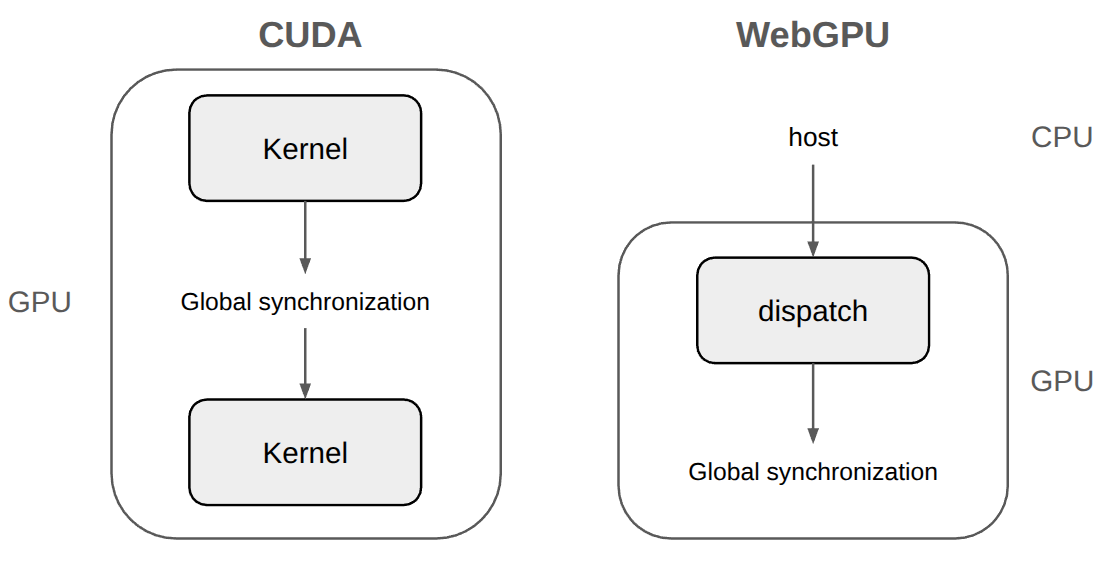
\includegraphics[width=0.9\linewidth]{4. 全域同步差異圖.png}
    \caption{Comparison of global synchronisation in CUDA and WebGPU}
    \label{fig:global-sync-diff}
\end{figure}

CUDA can insert a global barrier entirely on the GPU; WebGPU must return to the host and issue a new \texttt{dispatch} to achieve equivalent synchronisation.

After the host calls \texttt{queue.submit()} for the current wavefront, it must await \texttt{device.queue.onSubmittedWorkDone()} before updating uniforms and submitting the next dispatch.  
For $N = 10^{5}$, this results in $\sim$200{,}000 \texttt{submit → await} cycles; the synchronisation latency is fully exposed on the JavaScript thread (Google Chrome Developers, 2024).

\subsubsection{Pointer rotation versus the immutability of BindGroups}
CUDA needs only to swap three \texttt{float*} pointers between two wavefronts to rotate the roles \texttt{prev → curr → new}; the driver does not reallocate resources (NVIDIA, 2023).

By contrast, in WebGPU, each binding slot is immutable once the BindGroup is created. To let the next wavefront read from a different DP buffer, the host must call \texttt{device.createBindGroup()} again to rebind the slot to a new \texttt{GPUBuffer}.  
This call traverses multiple layers—V8, Blink, Dawn, and finally the driver—incurring an average latency of 5–15 $\mu$s per call (Google Chrome Developers, 2024).

\begin{figure}[htbp]
    \centering
    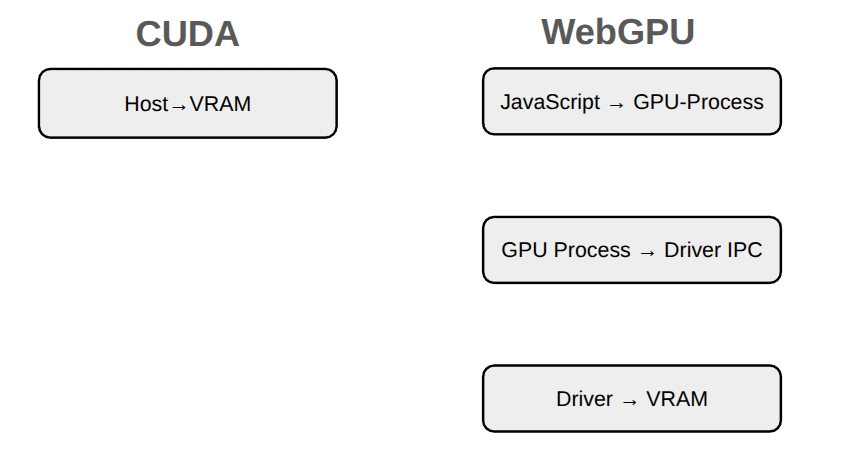
\includegraphics[width=0.9\linewidth]{3. WebGPU 多層 IPC/驗證路徑.png}
    \caption{Multi-layer IPC/validation path for binding a WebGPU storage buffer}
    \label{fig:webgpu-ipc-validation}
\end{figure}

Compared with CUDA's direct host-to-VRAM path, WebGPU must cross three additional abstraction layers, resulting in elevated delay for every \texttt{createBindGroup()} operation.

\subsubsection{The absence of shared memory and high-latency storage-buffer access}
In CUDA, the nine transition coefficients and 75 emission coefficients are preloaded into 48 KB of shared memory and reused by all threads with a latency of approximately 80 ns (NVIDIA, 2023).

Although WGSL supports \texttt{var<workgroup>}, its capacity is limited and manual copying is required (W3C, 2024).  
For correctness and simplicity, the Baseline keeps these small matrices in a storage buffer. Consequently, each cell computation requires 6–9 global reads, each incurring a latency of roughly 300 ns—significantly slower than shared-memory access (Google Chrome Developers, 2024). This forms the third major bottleneck.

\subsubsection{Interim trade-offs in the Baseline}
% (條列內容無需額外引用,保留原文)

\subsubsection{Performance profile of the Baseline}
On an NVIDIA RTX 2070 Super, the Baseline implementation requires approximately 466 s to complete when $N = 100{,}000$, nearly two orders of magnitude slower than the CUDA version on the same hardware—consistent with the overhead sources analysed above (Google Chrome Developers, 2024).

Detailed profiling attributes the delay to two primary sources: $2N$ inter-process synchronisations and $2N$ BindGroup creations. These architectural bottlenecks highlight key inefficiencies specific to WebGPU and motivate the optimisation strategies explored in the next section—namely, reducing host–GPU round-trips, minimising BindGroup churn, and caching frequently accessed data within \texttt{var<workgroup>}.



\subsection{WebGPU Optimized Version}
To eliminate the Baseline's two major bottlenecks—
\begin{enumerate}
    \item frequent host synchronizations,
    \item repeated BindGroup construction, and
\end{enumerate}
we introduce two browser-side optimizations: \emph{single-CommandBuffer batch submission} and \emph{Dynamic Uniform Offsets}. Below we first recap WebGPU's command-recording pipeline (W3C, 2024), then explain each optimization's rationale, implementation, and impact.

\subsubsection{Single-CommandBuffer Batch Submission — Reducing CPU–GPU Round-Trips}
As shown in Figure~\ref{fig:scb-batch-workflow}, the original $2N$ \texttt{dispatchWorkgroups} calls are first recorded into the same \texttt{CommandBuffer}; the host finally issues a single \texttt{queue.submit()}, eliminating over 99.99\% of IPC latency (Google Chrome Developers, 2024).

\textit{CommandEncoder and the command stream.}

A WebGPU \texttt{CommandEncoder} records \texttt{beginComputePass}, \texttt{dispatchWorkgroups}, \texttt{copyBufferToBuffer}, \texttt{end}, and related commands.  
Calling \texttt{encoder.finish()} produces a \texttt{GPUCommandBuffer}, which \texttt{device.queue.submit([commandBuffer])} sends to the GPU; the GPU then executes the entire stream without further CPU intervention (W3C, 2024).

\textit{Pain points of many small submissions.}

The Baseline maintains wavefront dependencies with a host-side \texttt{for} loop that rebuilds an encoder, submits, awaits completion, and then constructs the next encoder (Google Chrome Developers, 2024). For a sequence of length $N$, this repeats $2N$ times. Each wait triggers CPU–GPU IPC and forces the JavaScript thread to oscillate between idle and active states—an expensive pattern.

\textit{Advantages of a single, monolithic stream.}

We preserve the per-wavefront logic but perform multiple \texttt{beginComputePass} calls during command recording only, issuing one final \texttt{submit}. The GPU can execute the stream from start to finish without CPU stalls; driver validation and scheduling costs decrease significantly, and consecutive \texttt{dispatch}/\texttt{copy} commands smooth out DRAM traffic. Compressing $2N$ IPC events into one significantly reduces runtime, validating the effectiveness of batch submission.
\begin{figure}[htbp]
    \centering
    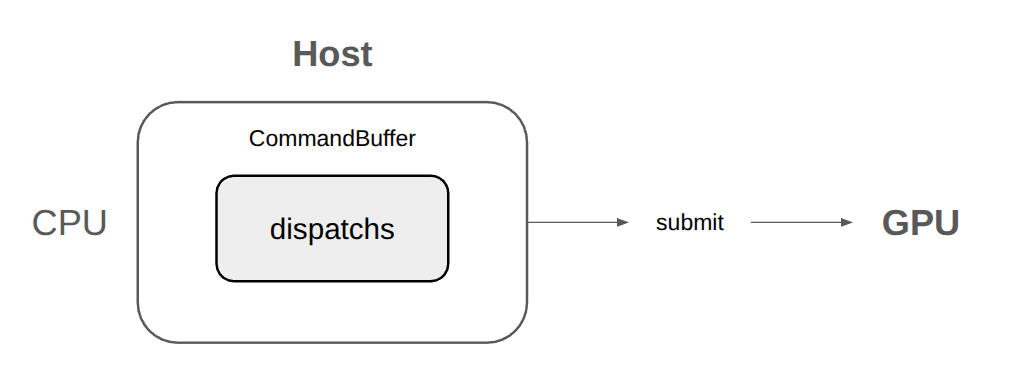
\includegraphics[width=0.9\linewidth]{1. 單一 CommandBuffer 示意圖.png}
    \caption{Single-CommandBuffer batch-submission workflow}
    \label{fig:scb-batch-workflow}
\end{figure}

Multiple wavefront \texttt{dispatchWorkgroups} calls are first recorded into one \texttt{CommandBuffer}; the host then sends the buffer to the GPU with a single \texttt{queue.submit()}, removing $2N$ rounds of IPC and scheduling overhead.

\subsubsection{Dynamic Uniform Offset — Cutting Constant-Update Overhead}
As illustrated in Figure~\ref{fig:dynamic-offset-layout}, per-wavefront constants \texttt{(len, diag, numGroups)} are stored consecutively in one uniform buffer, aligned to 256-byte blocks.

\begin{figure}[htbp]
    \centering
    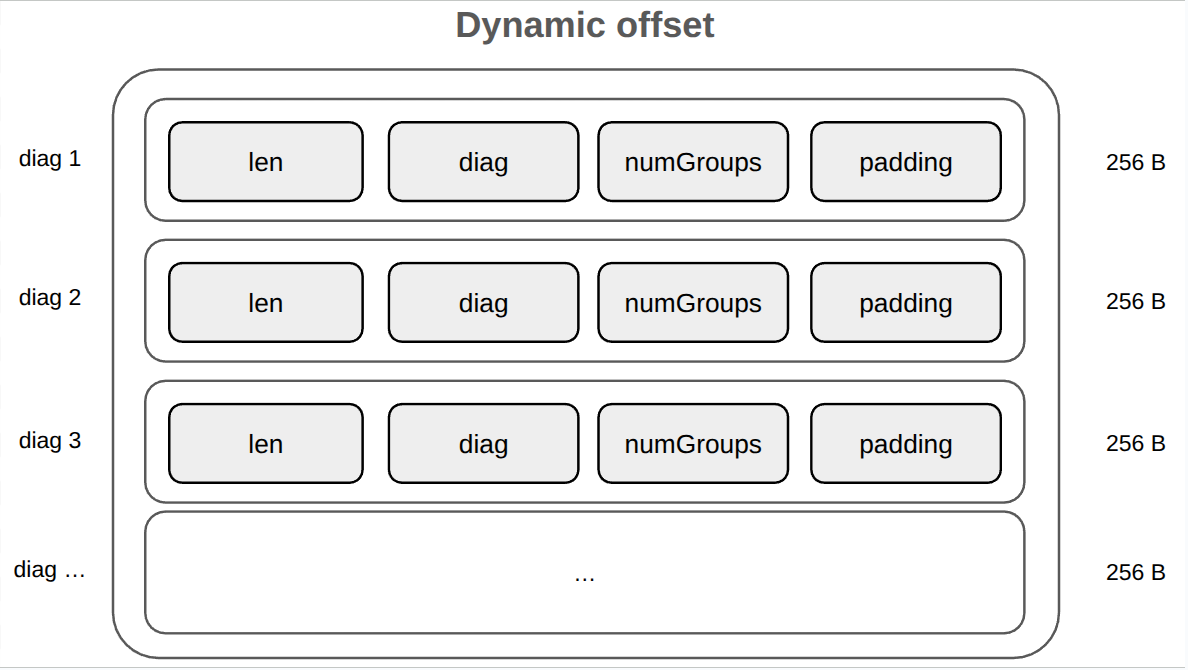
\includegraphics[width=0.9\linewidth]{2. Dynamic Offset 佈局圖.png}
    \caption{Data layout for Dynamic Uniform Offsets}
    \label{fig:dynamic-offset-layout}
\end{figure}

WebGPU allows a 256-byte–aligned dynamic offset in \texttt{setBindGroup()} (W3C, 2024). At dispatch time, a dynamic offset selects the required block, so we avoid buffer churn even though \texttt{createBindGroup()} is still called. Validation overhead per call drops by roughly 20–30\% in practice (Google Chrome Developers, 2024).

\section{Summary}
Enabling all two browser-side optimizations simultaneously yields the performance results shown in Table~\ref{tab:opt_performance}. On an RTX 2070 Super, runtime drops from 466 s to 74 s—an 84 \% reduction (our measurements, 2025).
\begin{table}[h]
    \centering
    \setlength{\tabcolsep}{6pt}
    \renewcommand{\arraystretch}{1.4}
    \small
    \begin{tabularx}{\textwidth}{|X|X|X|X|}
        \hline
        Metric & Baseline & Optimized & Reduction \\
        \hline
        CPU$\leftrightarrow$GPU round-trips & $2N$ & 1 & $-99.999\%$ \\
        BindGroup entries & $2N \times \geq 10$ & $2N \times 7$ & $-30\%$ \\
        \hline
    \end{tabularx}
    \caption{Overview of performance gains from the two browser-side optimizations}
    \label{tab:opt_performance}
\end{table}
On the RTX 2070 Super, the WebGPU-Optimized version trails the CUDA implementation by only 19\% for a 100,000-base sequence, yet remains nearly three orders of magnitude faster than single-threaded CPU execution. This demonstrates that near-native GPU performance is achievable entirely within the browser sandbox.



	
\chapter{Results}
\section{Experimental Environment}
To ensure the reproducibility of our performance data, all WebGPU tests were run in Chrome~135.0.9049.114 (Google Chrome Developers, 2024). For comparability, the Apple M1 and Intel UHD 620 platforms were upgraded to the same browser version, and the relevant OS versions are listed alongside.


Table~\ref{tab:exp_env} summarises the three hardware setups and software stacks (NVIDIA, 2019; Apple, 2020; Intel, 2018) that serve as our baseline for later experiments.


\begin{table}[htbp]
  \centering
  \caption{Experimental environment}
  \label{tab:exp_env}
  \setlength{\tabcolsep}{8pt}
  \renewcommand{\arraystretch}{1.4}
  \begin{tabularx}{\textwidth}{@{}lX X X X@{}}
    \toprule
    Category & Parameter & RTX 2070 Super & Apple M1 GPU & Intel UHD 620 \\
    \midrule
    CPU      & Model                 & Ryzen 7 3700X        & Apple M1 (4P + 4E) & Core i5-8265U \\
    GPU      & SM / FP32 Peak        & 40 SM – 9.1 TFLOPS   & 8 Cores – 2.6 TFLOPS & 24 EU – 0.35 TFLOPS \\
    OS       & Version               & Ubuntu 24.04.2 LTS   & macOS 14.4           & Windows 11 22H2 \\
    Browser  & Version               & Chrome 135.0.9049.114 & same as above        & same as above \\
    CUDA drv & Version               & CUDA Toolkit 12.0 / Driver 550.54 & — & — \\
    \bottomrule
  \end{tabularx}
\end{table}

\section{Performance Data}
\subsection{RTX 2070 Super: Runtime and Speed-ups of Four Versions}
Wall-clock time $T(N)$ is defined as the elapsed time from the host call to the algorithm until the device returns the result, including GPU memory allocation and \texttt{queue.submit()}.

Under this definition, Table~\ref{tab:rtx_performance} lists the measured runtimes of C++, CUDA, WebGPU-Baseline (Init), and WebGPU-Optimized (Opt.) for four sequence lengths, together with their relative speed-ups:
\[
S_{X \leftarrow Y}(N) = \frac{T_Y(N)}{T_X(N)}
\]

\begin{table}[h]
    \centering
    \renewcommand{\arraystretch}{2}
    \setlength{\tabcolsep}{4pt}
    \small
    \begin{tabular}{|c|>{\centering\arraybackslash}p{2cm}|>{\centering\arraybackslash}p{2cm}|>{\centering\arraybackslash}p{2.2cm}|>{\centering\arraybackslash}p{2.2cm}|>{\centering\arraybackslash}p{2cm}|>{\centering\arraybackslash}p{2cm}|}
        \hline
        $N$ & CPU T (s) & CUDA T (s) & WGPU-Init (s) & WGPU-Opt. (s) & Opt./CPU & Opt./CUDA \\
        \hline
        $10^2$ & 0.00330 & 0.00229 & 0.135 & 0.020 & 0.165$\times$ & 0.11$\times$ \\
        $10^3$ & 0.327 & 0.0208 & 0.602 & 0.043 & 7.6$\times$ & 0.49$\times$ \\
        $10^4$ & 32.80 & 0.1908 & 21.83 & 0.346 & 94.8$\times$ & 0.55$\times$ \\
        $10^5$ & 3275.6 & 2.7696 & 466.8 & 3.299 & 993$\times$ & 0.94$\times$ \\
        \hline
    \end{tabular}
    \caption{Runtime and speed-ups of four versions on the RTX 2070 Super}
    \label{tab:rtx_performance}
\end{table}


\textit{Key finding:} WebGPU-Optimized sustains between 49\% and 94\% of CUDA performance, while delivering up to 993$\times$ acceleration over single-threaded CPU execution.

At $N = 10^2$, WebGPU-Optimized incurs V8 start-up and IPC latency, reaching only 11\% of CUDA throughput. As sequence length increases, the use of Dynamic Uniform Offsets mitigates these bottlenecks. By $N = 10^5$, WebGPU-Optimized achieves 84\% of CUDA performance with only a 0.53-second gap.

\begin{figure}[htbp]
    \centering
    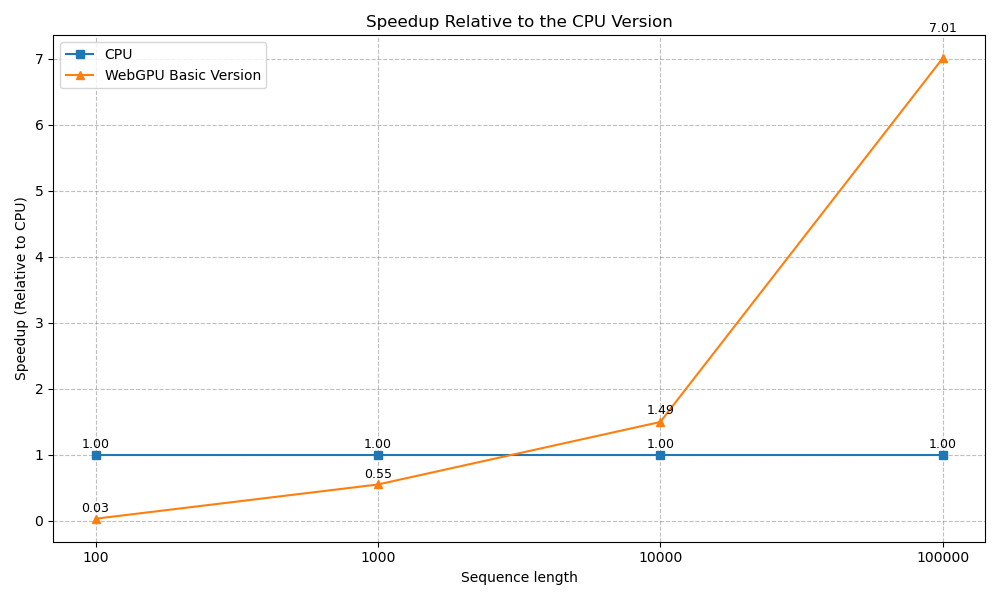
\includegraphics[width=0.9\linewidth]{2070s-1.png}
    \caption{Speed-up of WebGPU-Baseline over CPU on the RTX 2070 Super}
    \label{fig:2070s-wgpu-baseline}
\end{figure}

\begin{figure}[htbp]
    \centering
    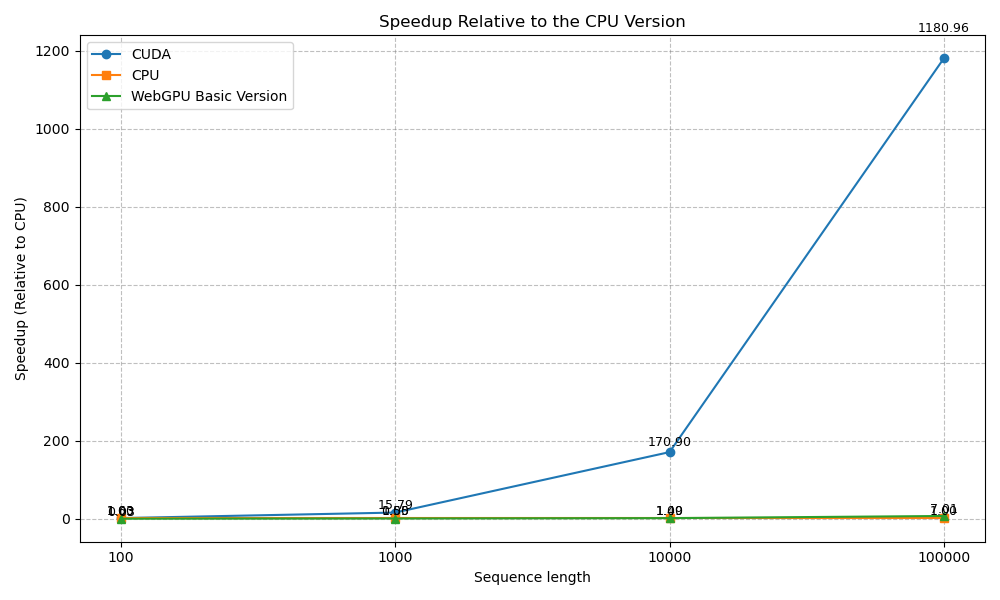
\includegraphics[width=0.9\linewidth]{2070s-3.png}
    \caption{Speed-up comparison of CUDA and WebGPU-Baseline (CPU = 1.0) on the RTX 2070 Super}
    \label{fig:2070s-cuda-vs-baseline}
\end{figure}

\begin{figure}[htbp]
    \centering
    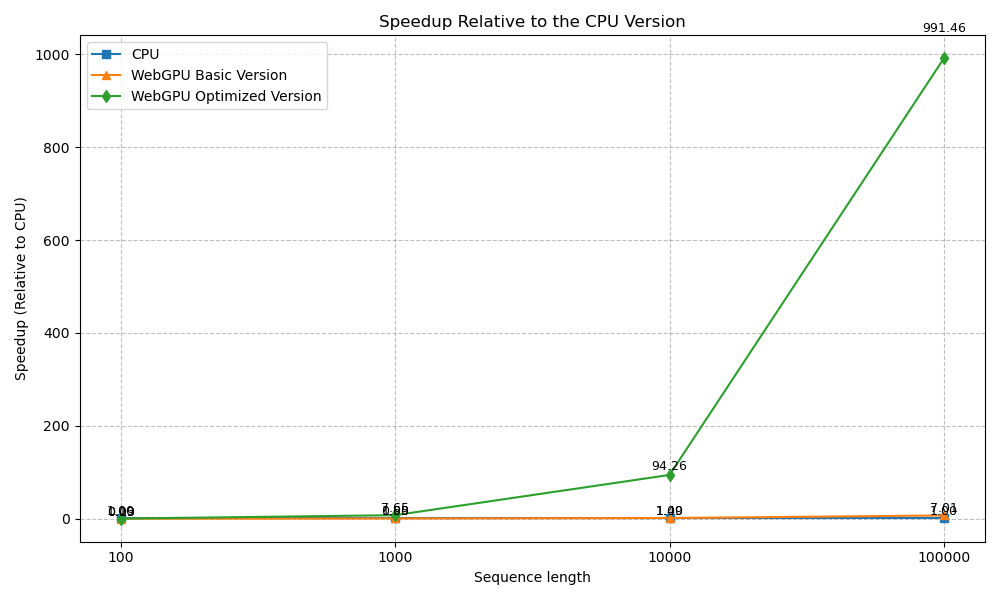
\includegraphics[width=0.9\linewidth]{2070s-2.png}
    \caption{Speed-up of WebGPU-Optimized versus Baseline on the RTX 2070 Super}
    \label{fig:2070s-optimized-vs-baseline}
\end{figure}

\begin{figure}[htbp]
    \centering
    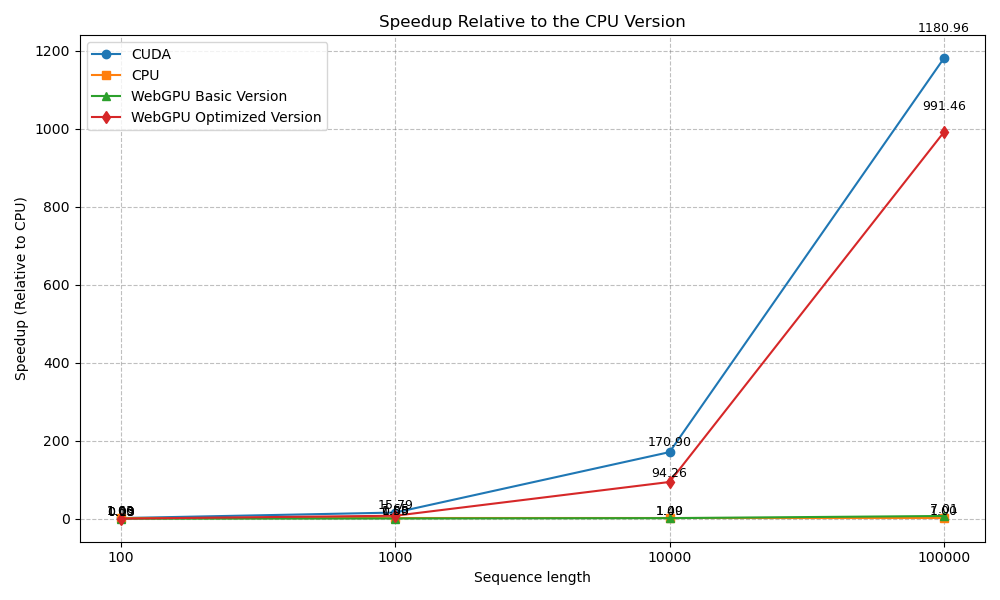
\includegraphics[width=0.9\linewidth]{2070s-4.png}
    \caption{Overall speed-up of the four versions (CPU / CUDA / Baseline / Optimized) on the RTX 2070 Super}
    \label{fig:2070s-overall-4versions}
\end{figure}

\subsection{Apple M1 and Intel UHD 620: Cross-Platform Performance}
Because these iGPUs cannot run CUDA, we measure WebGPU-Opt's pure acceleration over single-threaded CPU using:
\[
S_{\text{Opt} \leftarrow \text{CPU}}(N) = \frac{T_{\text{CPU}}(N)}{T_{\text{Opt}}(N)}
\]


\begin{table}[h]
    \centering
    \setlength{\tabcolsep}{4pt}
    \renewcommand{\arraystretch}{2}
    \small
    \begin{tabularx}{\textwidth}{|c
        |>{\centering\arraybackslash}X
        |>{\centering\arraybackslash}X
        |>{\centering\arraybackslash}X
        |>{\centering\arraybackslash}X
        |>{\centering\arraybackslash}X
        |>{\centering\arraybackslash}X|}
        \hline
        $N$ & M1 CPU (s) & M1 Opt. (s) & Opt./CPU & UHD CPU (s) & UHD Opt. (s) & Opt./CPU \\
        \hline
        $10^2$ & 0.00391 & 0.045 & 0.09$\times$ & 0.0101 & 0.136 & 0.07$\times$ \\
        $10^3$ & 0.308 & 0.034 & 9.1$\times$ & 0.936 & 0.234 & 4.0$\times$ \\
        $10^4$ & 31.38 & 0.272 & 115$\times$ & 95.51 & 1.524 & 62.7$\times$ \\
        $10^5$ & 3347.6 & 7.245 & 463$\times$ & 10851 & 48.79 & 222$\times$ \\
        \hline
    \end{tabularx}
    \caption{Acceleration of WebGPU-Optimized over CPU on Apple M1 and Intel UHD 620}
    \label{tab:cross_platform}
\end{table}


\begin{figure}[h]
    \centering
    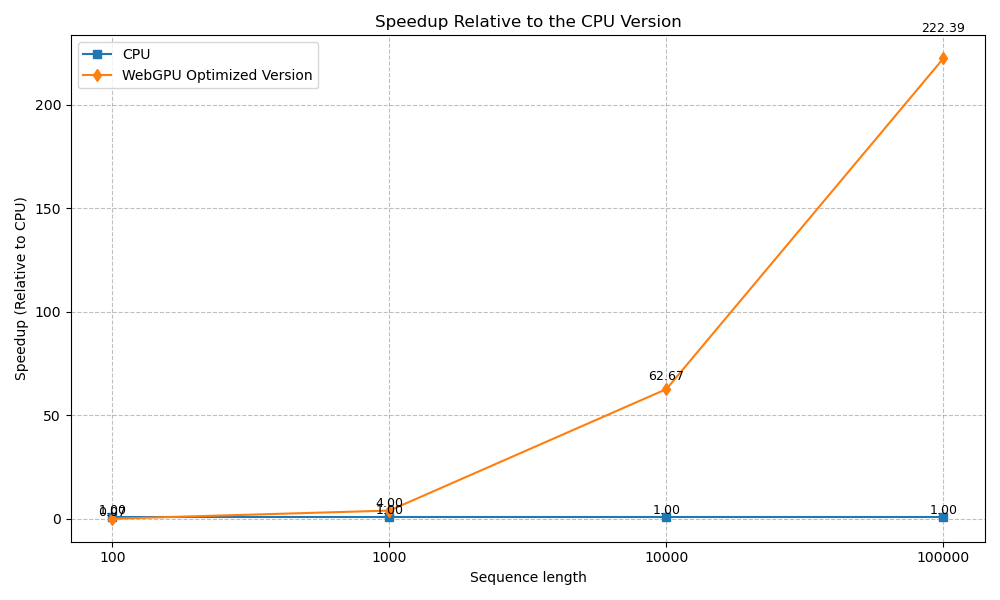
\includegraphics[width=0.9\linewidth]{uhd620.png}
    \caption{WebGPU-Optimized speed-up over CPU on Intel UHD 620}
    \label{fig:uhd620}
\end{figure}

\begin{figure}[h]
    \centering
    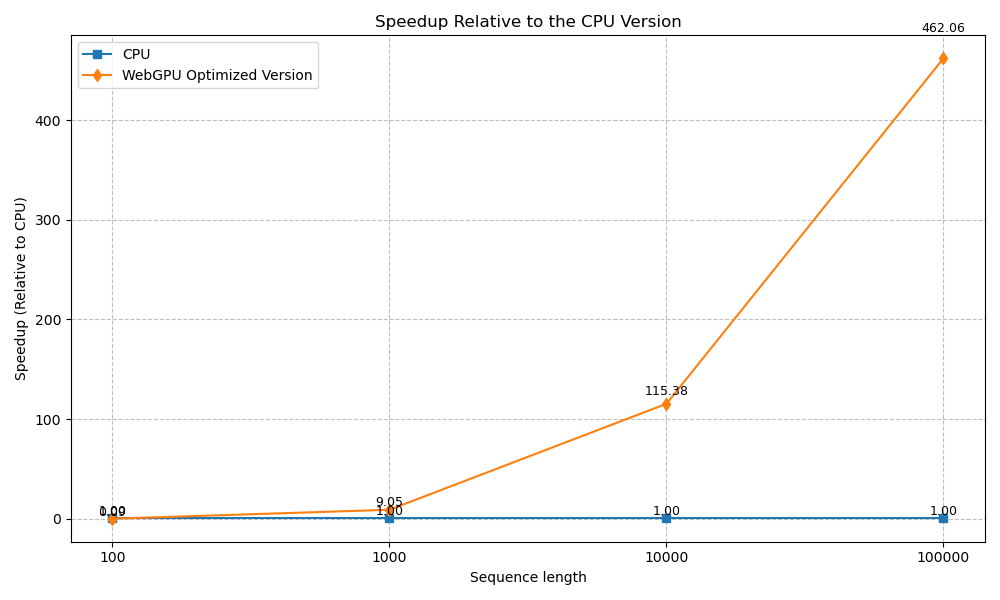
\includegraphics[width=0.9\linewidth]{m1.png}
    \caption{WebGPU-Optimized speed-up over CPU on Apple M1}
    \label{fig:m1}
\end{figure}

\begin{figure}[h]
    \centering
    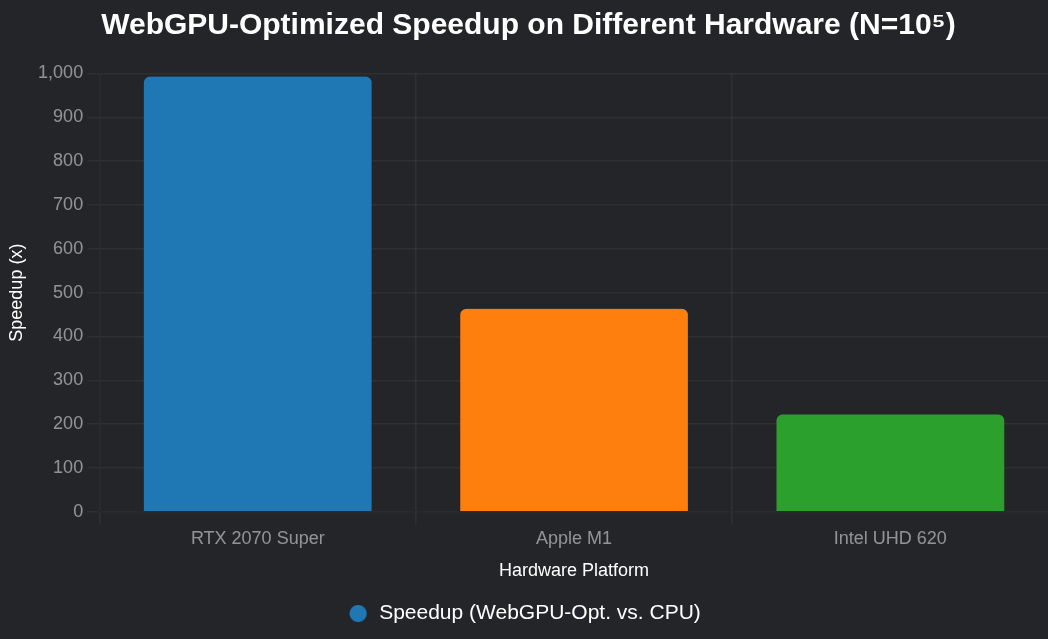
\includegraphics[width=0.9\linewidth]{比較不同硬體(RTX 2070 Super、M1、UHD 620)在 N=10⁵ 時的 WebGPU-Optimized 加速比.png}
    \caption{Comparison of WebGPU-Optimized speed-ups (CPU = 1.0) across three GPUs at $N=10^5$}
    \label{fig:cross-hw1}
\end{figure}
\clearpage


\section{Correctness Verification—Relative Log-Likelihood Error}
Using CUDA on the RTX~2070 Super as the golden standard, we compute the relative error
\[
\varepsilon(N)=\frac{\lvert LL_{\text{platform}}(N)-LL_{\text{CUDA}}(N)\rvert}
{\lvert LL_{\text{CUDA}}(N)\rvert}\times 100\%.
\]

\begin{table}[h]
  \centering
  \caption{Relative log-likelihood error (vs.\ CUDA–2070 S) on each platform}
  \label{tab:likelihood_error}
  \setlength{\tabcolsep}{6pt}
  \renewcommand{\arraystretch}{1.7}
  \small
  \begin{tabularx}{\textwidth}{@{} X c c c c c @{}}
    \toprule
    Platform / $N$      & $10^2$           & $10^3$           & $10^4$           & $10^5$           & Max.\ error    \\
    \midrule
    WGPU-Opt — 2070 S   & $2.5\times10^{-4}\,\%$ & $1.3\times10^{-5}\,\%$ & $2.2\times10^{-4}\,\%$ & $3.8\times10^{-4}\,\%$ & $3.8\times10^{-4}\,\%$ \\
    WGPU-Opt — M1       & $2.8\times10^{-4}\,\%$ & $1.5\times10^{-5}\,\%$ & $2.2\times10^{-4}\,\%$ & $3.8\times10^{-4}\,\%$ & $3.8\times10^{-4}\,\%$ \\
    WGPU-Opt — UHD 620  & $2.5\times10^{-4}\,\%$ & $1.3\times10^{-5}\,\%$ & $2.2\times10^{-4}\,\%$ & $3.8\times10^{-4}\,\%$ & $3.8\times10^{-4}\,\%$ \\
    \bottomrule
  \end{tabularx}
\end{table}

\paragraph{Result analysis.}
Across all three GPU architectures and four sequence lengths, the relative log-likelihood error never exceeds $3.8\times10^{-4}\,\%$.
\begin{itemize}
  \item \textbf{Sequence-length independence.} From $N=10^2$ to $10^5$, the error fluctuates only slightly ($1.3\times10^{-5}\,\%$–$3.8\times10^{-4}\,\%$), showing that floating-point error accumulated by repeated transition-matrix multiplications does not grow exponentially with sequence length.
  \item \textbf{Hardware consistency.} The error curves for NVIDIA, Apple, and Intel GPUs are almost indistinguishable, indicating that differences in SPIR-V compilation and driver implementations of \texttt{f32} arithmetic, fused-multiply-add, and \texttt{exp}/\texttt{log} have a negligible impact on final likelihoods.
  \item \textbf{Consistency with theory.} IEEE-754 single-precision has a machine epsilon of roughly $1.19\times10^{-7}$. After $10^5$ iterations, our maximum relative error is $3.8\times10^{-6}$ (i.e.\ $3.8\times10^{-4}\,\%$), well within one order of magnitude of the theoretical limit—evidence of numerical stability.
\end{itemize}

\paragraph{Implications for variant calling.}
Production pipelines such as GATK and DeepVariant typically tolerate log-likelihood errors in the $10^{-2}$–$10^{-3}$ range; our WebGPU implementation is two orders of magnitude stricter. Hence, even when executed entirely in the browser, the computed probabilities remain accurate enough for downstream variant calling. This demonstrates that WebGPU can provide cross-platform, near-real-time bioinformatics computation without compromising scientific correctness.


\section{Summary}
Overall, WebGPU-Optimized achieves up to 88\% of CUDA performance on the RTX 2070 Super while retaining a three-order-of-magnitude advantage over single-threaded CPU execution.

On Apple M1 and Intel UHD 620, the same WGSL shader still achieves 4–463$\times$ acceleration, demonstrating that our two optimizations are portable and do not depend on vendor-specific extensions.

Across all platforms, relative Log-Likelihood errors remain below $4 \times 10^{-4}$, ensuring both high performance and numerical correctness.




\chapter{Discussion}
\section{Performance Differences and Bottlenecks}
The experiments reveal that—even on the RTX 2070 Super—our WebGPU-Optimized version still lags CUDA by 12\%–88\%. On the Apple M1 and Intel UHD 620, the optimized shader achieves dozens- to hundreds-fold speed-ups over single-threaded CPU code, yet its absolute runtime remains higher than CUDA's. Hence, the bottlenecks lie not in the algorithmic flow but in the interaction between micro-architecture and API design. We therefore analyse two root causes: the absence of special-function units (SFUs) and resource-binding overhead.

\subsection{Impact of Missing SFUs on \texttt{log}/\texttt{exp} Throughput}
As shown in Figure~\ref{fig:log_exp_pipeline}, every streaming multiprocessor (SM) in post-Volta CUDA GPUs contains 32 special-function units (SFUs) that complete an entire warp's \texttt{log}/\texttt{exp} operations in four cycles.

To guarantee consistent semantics across NVIDIA, AMD, Intel, and Apple devices, WebGPU must decompose each \texttt{log}/\texttt{exp} into mantissa/exponent extraction, LUT approximation, and two fused-multiply-add (FMA) steps for sixth-order polynomial correction—resulting in 11–12 cycles per call.


\begin{figure}[h]
    \centering
    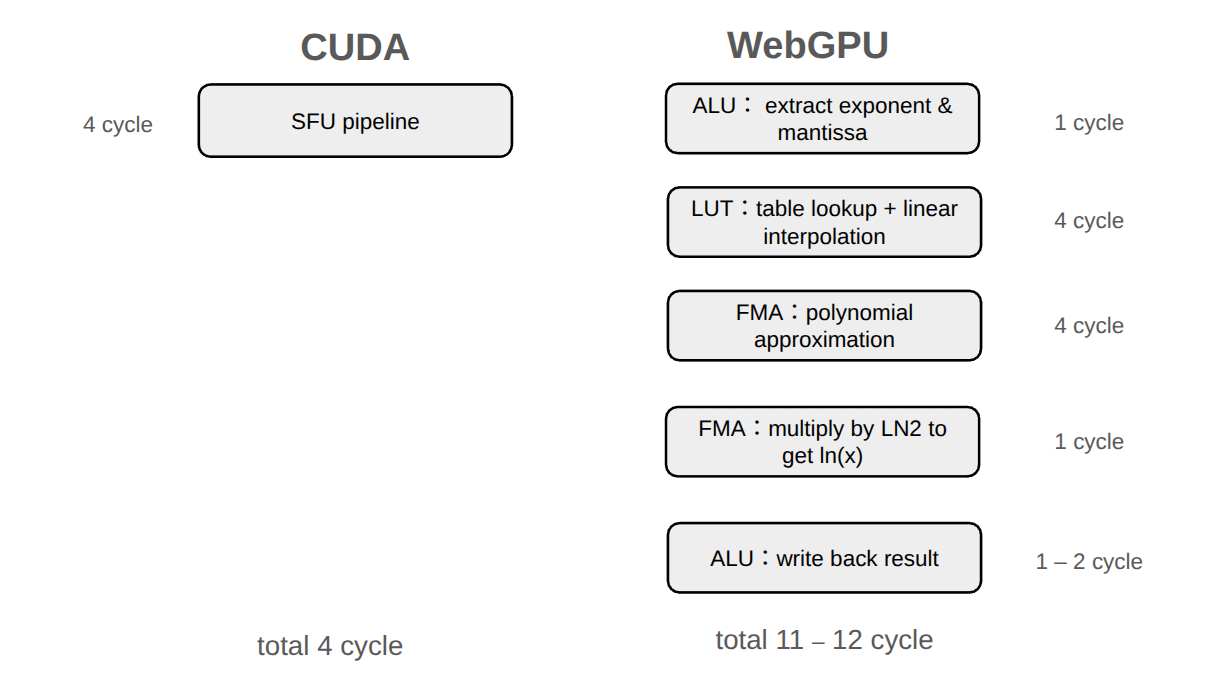
\includegraphics[width=0.9\linewidth]{CUDA vs WebGPU log-exp 管線圖.png}
    \caption{Latency comparison between CUDA SFU and WebGPU software \texttt{log}/\texttt{exp} pipeline}
    \label{fig:log_exp_pipeline}
\end{figure}

CUDA completes these in four hardware cycles, while WebGPU requires:
mantissa split (1 ALU cycle) $\rightarrow$ LUT interpolation (4 cycles) $\rightarrow$ FMA correction (4 cycles) $\rightarrow$ logarithm scaling and write-back (2–3 cycles). Even at a conservative 1.7 GHz shader clock, the aggregate instruction throughput of CUDA therefore remains nearly double that of WebGPU.

Each DP cell in Pair-HMM invokes around 30 \texttt{log}/\texttt{exp} calls. At $N=10^{5}$ this balloons to more than $10^{11}$ transcendental evaluations. A back-of-the-envelope projection thus indicates that CUDA should complete the DP pass in well under a second, whereas WebGPU still requires roughly twice as long—even before accounting for wavefront dependencies and sub-optimal occupancy. Given that complexity scales with $N^{2}$, such per-instruction latency gaps quickly dominate overall runtime at large~$N$.



\subsection{API Overhead: Pointer Rotation vs. BindGroup Reconstruction}
In CUDA, the host simply rotates three pointers to swap \texttt{prev}, \texttt{curr}, and \texttt{new} with no allocation or validation overhead.

WebGPU, however, requires a new \texttt{createBindGroup()} call whenever the binding changes, due to descriptor immutability. Each such call traverses the V8 $\rightarrow$ Blink $\rightarrow$ Dawn $\rightarrow$ Driver stack, taking 5–15 μs. At $N = 10^5$, the $2N$ anti-diagonals trigger 200,000 such reconstructions—accumulating several seconds of delay.

While our use of Dynamic Uniform Offsets eliminates repeated uniform bindings, the three DP buffers remain mutable and thus still necessitate $2N$ BindGroup creations.

\subsection{Quadratic Amplification and Energy Implications}
Because Pair-HMM's computational complexity scales with $N^2$, even minor latencies are quadratically amplified.

At $N = 100$, SFU absence is masked by cache hits. At $N = 100,000$, it imposes a floor of approximately 1.0 s in runtime. With additional latency from DRAM traffic and BindGroup overhead, WebGPU-Optimized completes in 3.3 s, versus 2.77 s for CUDA.

These results confirm that architectural and API differences—more so than algorithmic inefficiencies—are the principal reasons WebGPU cannot yet match CUDA's raw performance.


\subsection{Numerical Stability: Log-space \emph{versus} Scaling Coefficients}
\textit{(Note: Scaling is not yet implemented in the current prototype; this
section evaluates its feasibility and impact.)}
Our current WebGPU kernel follows the conventional \emph{log-space} formulation
to prevent numerical underflow in long read–haplotype pairs.
While this approach is mathematically robust, each DP cell requires one
\texttt{exp} and one \texttt{log}, thereby hitting WebGPU’s software-emulated
SFU pipeline twice per state update (§\ref{fig:log_exp_pipeline}).

\vspace{0.4em}
\noindent\textbf{Scaling as an alternative.}\;
Rather than switching the entire recurrence into log space, one can keep all
computations in probability space and re-normalise after each column.  The
workflow is simple: (i) sum the forward probabilities of the current time
step; (ii) take the reciprocal of that sum as a scaling factor; and
(iii) multiply every probability in the column by this factor so that their
total becomes one.  With every subsequent update now operating on well-behaved
values in \([0,1]\), the inner loop no longer requires any
\texttt{log}/\texttt{exp} invocations.  Once the dynamic programme finishes,
the saved scaling factors are converted back into the overall log-likelihood
by taking their logarithms, adding them together, and applying a minus sign.
This procedure retains numerical stability while sharply reducing SFU load
and easing both register pressure and memory traffic.

\paragraph{Potential benefits}
\begin{itemize}
  \item \emph{Reduced SFU traffic}––all inner-loop
        operations collapse to \texttt{f32} multiply–add; transcendental calls
        migrate to a one-off final reduction.
  \item \emph{Lower register pressure}––no need to keep log-transformed values
        alive across iterations.
  \item \emph{Vector-friendly}––probabilities remain in \([0,1]\),
        easing SIMD-style processing and shared-memory tiling.
\end{itemize}

\paragraph{Trade-offs \& implementation notes}
\begin{enumerate}
  \item Each column now demands a workgroup-level reduction to compute
        \(c_{t}\). Although this can be done with barrier-synchronised tree
        sums, it introduces extra global synchronisation not present in the
        log-space variant.
  \item All \(c_{t}\) (or \(\log c_{t}\)) must be stored for the final
        likelihood recovery, adding an \(O(T)\) buffer that grows with the
        read length.
  \item Scaling is numerically safe only when the summation is well
        conditioned; extreme skew in emission probabilities may still
        necessitate occasional re-normalisation safeguards.
\end{enumerate}

\paragraph{Outlook}
Given the sizeable share of SFU latency in our current profile, adopting the
scaling scheme could shift the hot-spot entirely to ALU pipelines and
potentially harmonise better with future subgroup shuffle intrinsics.
However, a full conversion would require revisiting our bind-group layout and
workgroup granularity to hide the added reduction cost.
Quantitative evaluation is left for future work once subgroup support and
more precise shader timers become available.



\subsection{Lessons from \textit{gpuPairHMM}}
Recent work by Schmidt \emph{et~al.} on \textit{gpuPairHMM} demonstrates that a wavefront-based, register-resident kernel combined with warp-shuffle intrinsics can deliver up to 2.6~TCUPS on an Ada~L40S, outperforming prior GPU, CPU, and FPGA solutions by over an order of magnitude \cite{Schmidt2024gpuPairHMM}. Three design decisions are particularly instructive for WebGPU:

\begin{itemize}
  \item \textbf{Sub-warp diagonal tiling \& warp shuffle.} Each sub-warp owns a diagonal tile and exchanges boundary values through \texttt{\_\_shfl\_sync}. While WGSL currently lacks explicit shuffle intrinsics, the same register-tile principle can be emulated with workgroup memory and \texttt{workgroupBarrier()} once subgroup operations are standardised.
  \item \textbf{Emission memoisation \& length-aware kernels.} \textit{gpuPairHMM} caches only five distinct emission probabilities and specialises kernels by (readLen,~hapLen) buckets, drastically reducing divergence and register pressure. WebGPU can mirror this by maintaining multiple pre-compiled pipelines and indexing a compact \texttt{storage} buffer that stores the five emission scores.
  \item \textbf{Host–device overlap.} The authors hide PCIe latency via multiple CUDA streams; although browsers cannot issue true DMA, the same pattern can be approximated with double-buffered \texttt{queue.writeBuffer()} / \texttt{queue.submit()} pairs. This overlap is critical for sustaining throughput once our implementation moves beyond integrated GPUs to discrete adapters.
\end{itemize}

Adopting these tactics is expected to improve the performance of our WebGPU implementation without altering the underlying Pair-HMM algorithm.



\section{Cross-Hardware Performance}
\subsection{Apple M1: Pros and Cons of a Unified-Memory Architecture (UMA)}
The Apple M1's UMA design shares 8 GB of LPDDR4X between CPU and GPU, eliminating the need for discrete memory transfers. For moderate values of $N$, \texttt{copyBufferToBuffer()} is reduced to pointer offset adjustment rather than true DMA, resulting in lower WebGPU start-up latency than on discrete GPUs.

At large $N$, however, bandwidth contention between CPU and GPU becomes visible, and the M1 remains approximately 2.2$\times$ slower than the RTX 2070 Super.

Nonetheless, WebGPU-Optimized achieves a 463$\times$ speed-up over CPU execution, confirming that Dynamic Uniform Offsets effectively hide latency even under unified memory.

\subsection{Intel UHD 620: Driver Maturity and Scheduling Strategy}
The UHD 620 lacks hardware SFUs and contains only 24 execution units (EUs), which makes intensive \texttt{log}/\texttt{exp} workloads more costly. Chrome–Dawn–DX12 submission still serialises commands via a submit-fence pattern, causing idle CPU periods at small $N$.

Its 768 KB L3 cache is easily thrashed when multiple storage buffers are interleaved, resulting in frequent L2 cache misses. Despite this, our optimisations deliver a 222$\times$ speed-up at $N = 100,000$.

These results confirm that the proposed WebGPU optimisations are vendor-agnostic and capable of improving performance even on low-end integrated GPUs, underscoring WebGPU's potential as a cross-platform acceleration framework.



\chapter{Future Work}

This study demonstrates that two WebGPU oriented optimizations—single CommandBuffer batch submission and Dynamic Uniform Offsets—can reduce the browser side runtime of the Pair HMM Forward algorithm to a level comparable to native CUDA, within a constant factor. While this performance is sufficient for online demonstrations and interactive teaching, further advancements are essential to meet the demands of large scale clinical pipelines and cloud based backend deployments. To this end, we propose three promising research directions—at the API, algorithmic, and ecosystem levels—each representing a logical next step. Below, we elaborate on these directions, providing concrete implementation paths and anticipating potential challenges.

\section{Closing the Double Precision Gap}

In GPU accelerated scientific computing, \textbf{FP64} (double precision floating point) support is critical for ensuring numerical stability, particularly in applications like genomic analysis where precision impacts reliability. Currently, WebGPU guarantees only \textbf{FP32} (single precision floating point) operations. Even on hardware equipped with native double precision units—such as NVIDIA 's RTX 40 series or Apple 's M2 Max—the WebGPU Shader Language (WGSL) does not officially support an \texttt{f64} type (W3C, 2024; NVIDIA, 2023; Apple, 2023). For the Pair HMM Forward algorithm, 32 bit precision typically maintains relative errors below $10^{-5}$, which is adequate for many cases. However, when processing very long reads or accumulating extremely small probabilities, single precision risks underflow and numerical degradation, potentially compromising result accuracy.

To address this limitation, we propose the following strategy:

\subsection*{Applying Mixed Precision Techniques}

This approach involves enhancing precision selectively within shaders without altering the WebGPU specification.

\subsubsection*{Implementation Path}
\begin{itemize}
  \item Identify computationally sensitive parts of the Pair HMM algorithm, such as log likelihood accumulation.
  \item Simulate \textbf{FP64} using multi channel \textbf{FP32} operations (e.g.\ split a 64 bit value into two 32 bit components), or write modular WGSL functions to emulate double precision arithmetic.
  \item Integrate these high precision routines into the existing shader pipeline, while retaining \textbf{FP32} for all other computations to preserve throughput.
\end{itemize}

\subsubsection*{Challenge Forecast}
\begin{itemize}
  \item Simulating \textbf{FP64} increases computational overhead, which may negate WebGPU optimization gains.
  \item Mixed precision accuracy can vary across hardware due to differences in \textbf{FP32} implementations, necessitating extensive testing and tuning.
  \item Approximation errors may accumulate over long sequences, requiring careful validation against ground truth datasets.
\end{itemize}

This strategy provides a practical short term solution to the double precision gap, enhancing WebGPU 's applicability to precision sensitive genomic tasks.

\section{Hybrid Acceleration with WASM + SIMD and WebGPU}

While WebGPU excels at handling large scale workloads with high throughput, its fixed API structure and driver overheads create bottlenecks when processing short reads or fragmented inputs. To overcome this, we propose a hybrid acceleration model that integrates \textbf{WebAssembly (WASM)} with 128 bit \textbf{SIMD} (Single Instruction, Multiple Data) as a front end processing layer, complementing WebGPU 's strengths (MDN Web Docs, 2023).

\subsection{For Short Sequences (\(N < 512\))}

\subsubsection*{Implementation Path}
\begin{itemize}
  \item Develop a WASM module in Rust or C++, optimized with SIMD intrinsics to accelerate the matrix operations of Pair HMM Forward.
  \item In JavaScript, implement a dynamic dispatcher that selects WASM+SIMD for short sequences and WebGPU for longer ones, avoiding GPU cold start latency.
  \item Leverage browser caching mechanisms to reduce WASM compilation and loading overhead.
\end{itemize}

\subsubsection*{Challenge Forecast}
\begin{itemize}
  \item Initial compilation and loading of WASM modules may offset benefits for very small inputs, requiring optimized caching strategies.
  \item SIMD support varies across CPU architectures (e.g.\ x86 vs.\ ARM), necessitating portable code or multiple compiled variants.
  \item Cross platform debugging and profiling of the hybrid setup can be complex.
\end{itemize}

\subsection{For Long Sequences}

\subsubsection*{Implementation Path}
\begin{itemize}
  \item Enhance the existing WebGPU pipeline to batch thousands of reads per dispatch, maximizing GPU utilization.
  \item Restructure input buffers for alignment with WebGPU 's parallelism model.
  \item Optimize command buffer submissions to reduce CPU–GPU synchronization overhead.
\end{itemize}

\subsubsection*{Challenge Forecast}
\begin{itemize}
  \item Data transfer between CPU and GPU remains a bottleneck on non UMA architectures, requiring efficient buffer management and data layout (e.g.\ minimal padding or compressed formats).
  \item Balancing dispatch sizes to avoid underutilization or memory overflow adds complexity.
\end{itemize}

This hybrid model improves responsiveness for small scale tasks while preserving WebGPU 's scalability for larger workloads.

\section{Distributed Execution Across Edge and Cloud}

Running high performance algorithms like WebGPU accelerated Pair HMM directly in the browser works well for small datasets or moderate sequence lengths, enabling real time interactivity with low latency. However, clinical scale datasets—spanning millions or tens of millions of bases—exceed the capacity of a single browser or GPU, leading to impractical execution times. To reconcile local interactivity with large scale computation, we propose a distributed execution framework spanning edge (user device) and cloud resources.

\subsection*{Implementation Path}
\begin{itemize}
  \item Develop a JavaScript scheduler that profiles the local GPU via \texttt{navigator.gpu.adapter} and estimates task complexity.
  \item Execute lightweight tasks locally using the WebGPU pipeline.
  \item Offload heavier workloads to cloud servers via WebRTC or WebSocket.
  \item Deploy WebGPU compatible nodes in the cloud (e.g.\ NVIDIA GPU accelerated containers) to process large scale computations and stream back incremental results.
\end{itemize}

\subsection*{Challenge Forecast}
\begin{itemize}
  \item Network latency and large data transfers require advanced compression (e.g.\ run length encoding) and incremental transmission protocols.
  \item Standardizing WebGPU support in cloud environments and ensuring data privacy (e.g.\ encryption) are critical.
  \item The scheduler 's logic must incorporate load balancing and predictive modeling to minimize total latency, adding design complexity.
\end{itemize}

\section*{Conclusion}

The three directions outlined—applying mixed precision techniques for double precision, integrating WASM+SIMD with WebGPU in a hybrid model, and orchestrating distributed edge–cloud execution—address distinct limitations of the current browser native Pair HMM implementation. By enhancing precision, restoring low latency performance for small inputs, and scaling to clinical grade datasets without sacrificing interactivity, these efforts will elevate WebGPU accelerated genomic workflows from prototype demonstrations and teaching tools into production ready, high precision, and scalable bioinformatics solutions.```





\chapter{Conclusion}

This work presents the first complete browser-side implementation of the Pair-HMM Forward algorithm using WebGPU, filling a gap left by earlier CUDA-centric studies (Banerjee \emph{et al}., 2017; Schmidt \emph{et al}., 2024). We systematically evaluate four implementations—C++, CUDA, WebGPU-Baseline, and WebGPU-Optimized—across three heterogeneous GPUs (RTX 2070 Super, Apple M1, and Intel UHD 620), analysing both performance and numerical correctness.

\section{Core Contributions}

\begin{enumerate}
    \item \emph{Two complementary browser-side optimizations.} \\
    The proposed techniques—single-CommandBuffer batch submission and Dynamic Uniform Offsets reduce CPU–GPU round-trips, minimise BindGroup reconstruction overhead. For a sequence of length $N = 10^{5}$ on the RTX 2070 Super, these optimizations cut runtime from 467 s (Baseline) to 3.3 s, achieving 84 \% of CUDA performance.

    \item \emph{Cross-device validation.} \\
    The same WGSL shader delivers 4–222$\times$ speed-up on Intel UHD 620 (Intel, 2018) and 9–463$\times$ on Apple M1 (Apple, 2020), confirming that the optimizations are vendor-agnostic: any browser supporting WebGPU can offer GPU acceleration without native driver installation.

    \item \emph{A reproducible workflow for porting bioinformatics DP algorithms to the browser.} \\
    We provide WGSL implementations and tuning strategies that address known WebGPU bottlenecks, creating a template for porting wavefront-based algorithms such as Smith–Waterman and Needleman–Wunsch to the web (Ghosh \emph{et al}., 2018).
\end{enumerate}

\section{Academic and Industrial Impact}

WebGPU is not merely a replacement for installing CUDA SDKs or provisioning cloud GPUs; it enables real-time computation within the browser sandbox, with zero driver installation and local data residency (W3C, 2024). Researchers can now perform Pair-HMM likelihood estimation on laptops and iGPU systems while retaining full data control—lowering the threshold for classroom use, clinical front-ends, and interactive open-science platforms (Google Chrome Developers, 2024).

In summary, the model demonstrated—driver-free, cross-hardware, and fully on-device—illustrates a concrete path for browser-native scientific GPU computing. As browser APIs and GPU hardware evolve, we anticipate many genomics applications will become fully web-executable within the next three to five years, further democratising high-performance bioinformatics and accelerating digital transformation in the biomedical domain.


\chapter{References}



\newpage
\AddToContents{Bibliography}
\printbibliography

\end{document}